\chapter{Simulation}
\label{simulation}
{}To evaluate different strategies when evolving a component system, the environment in which these evolutions occur is simulated.
{}Through modelling then simulating the different aspects of a system; the user-interaction, the repository, and the resolver;
{}conclusions can be drawn on the benefits and draw backs of a particular evolution strategy.

{}The motivations for simulating and the methodology used to create the simulation are presented in this chapter.
{}The result of this chapter is a simulation that can be used to predict how a component system will evolve given different variables of the user and the strategy they use.

\section{Why Simulate?}
%%%Why are we using a simulation instead of real systems, or a controlled environment
To evaluate an evolution strategy some options include;
using a set of actual systems with real users could be accessed to collect field data;
creating a controlled environment in which users are given tasks and monitor the outcomes;
simulating a systems evolution through creating models and altering environment variables to study their effects.
In this section we discuss the positive and negative aspects of each of these approaches,
and present the reasons for the selection of the simulation methodology for this research.

\subsection{Using Real Users and Systems}
%%%The pros and cons of using real systems with real users
Using real systems with real users would clearly produce real and valid data to be studied and analysed to find the best evolution strategies.
Solvers could be developed and distributed to different users, each solver using different criteria 
and as each user has different behaviours (amount they install, when they update)
these results could be analysed to find strategies that produce good systems. 

%%%Now the cons
This approach will create very accurate research, however it has some significant drawbacks,
it will take significant periods of time to create meaningful results, for each day of results you have to wait a day.
Finding the way a particular strategy effects a system over an entire year, will mean waiting a year.
More significantly, finding users that will trust an experimental system to alter their real system would be extremely difficult.   
A user will likely not trust a newly released resolver, as their system is important to them and even the slightest error can cause
a system to become unstable.

%%%Users trust is difficult to gain
To gain the trust of possible users the experimental resolvers would have to be thoroughly tested through a repositories development cycle and be well maintained.
Moving a package through this cycle can be itself a massive undertaking lasting several months. 
For example Eclipse Plug-ins it involves going a component going through four phases 
Proposal, Incubation, Mature, and Top-Level\footnote{http://www.eclipse.org/projects/dev\_process/development\_process\_2010.php};
similar to Debian's process of moving through the phases Unstable, Testing, Frozen, and finally stable\footnote{http://en.wikipedia.org/wiki/File:Debian-package-cycl.svg}.
After it has been through this cycle, maintenance of the resolver is still required; 
for instance the Ubuntu package ``apt'' has released about 2 changes a month\footnote{http://changelogs.ubuntu.com/} to it or related packages since its initial release.
This shows how much effort must be applied to earn a users trust, and this effort will likely outweigh the actual benefits.

\subsection{Real users in a Controlled Environment}
%%%The pros and cons of using real users with pseduo systems
A study of users interacting with a system in a monitored and controlled environment could be executed.
Each user could be given different strategies, e.g. solver criteria, and different tasks to perform on their system to approximate real interactions.
This study could compress a years worth of interactions with a system into an hour, and produce results from real users. 
Compared to the previous type of study using real users with real systems,
this research removes the necessity of user trust as the user is altering a system that is not theirs,
and results can be gained in hours not years. 
However, it will also produce less valid results, as it is still an approximation of a real system, and the users know this.
Any controlled environment would alter how the user interacts with their controlled system, making the results less reliable.
For example, a user typically researches a package before selecting installing it because it would have real implications, 
in a controlled environment these implications are removed so the selection would still be of questionable validity.

The largest problem with this method is again finding enough users.
With the previous method it was trust that would limit the user count, here it is the effort to find and monitor the amount of necessary users required.
For example, given we want to test 10 different strategies with 5 different user types, each combination must contain multiple different test subjects to find statistically significant results, 
and each subject taking upwards of an hour to complete the study. 
This would be a significant effort to organise users, monitor interactions and collect results, so much so that that it may be logistically impractical when compared to the benefits.


\subsection{Using a Simulation}
%%%Instead we can simulate, with an approximation of the real world.\\ 
%%%When drawing conclusions the accuracy of this approximation must be considered, therefore significant effort has gone into data collection and validation.
A simulation is a surrogate of the real system, such that it represents the core aspects of a component systems evolution.
This is accomplished through modelling the most important parts of the system, 
and computationally creating and measuring the results. 
As the simulation is only an approximation of the real world, 
the accuracy to which it actually represents the real world is not 100\%.
The goal is then to make it a ``close enough'' approximation so that the conclusions drawn from it are valid in the real world.
So when analysing the results and forming conclusions, we must take into account the assumptions we have made creating the simulation to determine 
the conclusions overall accuracy.
Therefore, the majority of the effort when creating a simulation is gathering and using valid information when making assumptions.

%%%What is good about the simulation over the other two methods, speed at which results are generated, the cost to get the results, the control over the variables in the simulation.
Simulation is superior to either using real users and real systems, or using a controlled environment in the speed at which hypotheses can be tested and evaluated,
the cost to test and get results, and the control over variables and configuration of the environment.

%%%Speed at which results are generated
As the speed increases at which a hypothesis can go from being an idea on paper to being tested in a real or simulated environment, increased the amount of meaningful information can be generated. 
When an idea is proposed as a possible solution to a problem, the quicker that idea can be eliminated or encouraged allows new ideas to be formed off of the original.
These ideas themselves can then be tested, to see if they are suitable solutions.
The faster this process is, the ideas can be tested, the better solutions and more information is generated.
Using real users, or real systems, requires long periods of waiting, where if the actions and environment can be modeled and executed computationally there is little waiting.
Through simulation an idea can be tested almost immediately by simultaneously evolving multiple simulated systems, where using a real user, 
it may take days or months to generate the same amount of results.  

%%%Cost
The cost of using any of these methods can be measured in the amount of time it would take in organising, measuring and wasted time, for the the results to be collected.
Using a real user and system would involve an enormous amount of time validating and distributing the solvers (as discussed earlier), 
and the controlled environment would require many hours of organisation and planning to gather the necessary users, and then measure their interactions with the system.
However, with a simulation the main effort is ensuring that the models are accurate enough to gather meaningful results.
This time in validating the simulation and associated models is only necessary once, 
i.e. if more results are needed the simulation will not need to be re-validated.
The other two methodologies do not have this property, as for each user tested and measured will be a duplicate effort. 

%%%Control
The control over the results that a simulation returns far exceeds the other methods as models can be altered and tested where a real user cannot. 
This control allows the testing of extreme situations, the sensitivity analysis of different variables,
and the generation of possibly optimal but 'out of the box' ideas. 
For instance, the testing of the amount of days a user waits between updates can be tested through altering the times between updates, then running the simulation.
If real users where used, the amount of users necessary to be collected would be enourmous to produce any significant results in this area.

%%%Final words on why we simulate
A simulation was used as it provides us with a cost/benefit ratio that is desirable, while potentially allowing an appropriate level of accuracy to draw meaningful conclusions.
The main effort is then to create the simulation with valid models that will give us the desired accuracy.

\section{Methodology}
%%%We use the methodology from `` Build a Valid and Credible Simulation''
{}A goal of this study is to create a reusable simulation for future use, and to provide useful information on the process of component evolution. 
{}This places validity and credibility of a simulation and the results it provides at a high priority.
{}To create such a simulation the methodology outlined by \cite{Law2005} in ``How to build valid and credible simulation models'' is followed.
{}This methodology is a guideline for defining the study, collecting information, creating and validating models, and running the simulation.
{}In this section we introduce the methodology with its goals and how they are aligned to ours, 
{}discuss the steps that it recommends to be taken to create a valid simulation, and how the simulation will be created and what it will produce for this study.

\subsection{Validation and Credibility}
%%%Why do we use this methodology and how is it relevant?
This methodology was created after the observation that validation was often ``attempted after the simulation models had already been developed'',
and that the validation may of only occurred only if there was money and time left at the end of the project.
However, such simulations, that are not validated, can produce erroneous information that leads to incorrect, possibly costly and bad decisions being made.
This reduces the credibility of the simulation to be used in future as a tool.

%%%What is a valid simulation?
A simulation is an abstraction and simplification of reality, usually created as using an actual system can be disruptive, not cost-effective, or simply impossible.
In this context ``\textit{Validation} is the process of determining whether a simulation is an accurate representation of the system, for the particular object of the study.''
So a valid simulation if an abstraction that accurately represents a system closely enough for an objective of a study to be completed.
The later part is an important aspect of validation, as the accuracy of the simulation is directly dependent on the problem and questions the study addresses.
A simulation that is 99\% accurate may cost significantly more to produce than one that is 90\%, but provide little additional benefit given the specific information wanting to be gained from it.
Therefore an important aspect of the simulation is the definition of the problem, as it will lead to the definition and scope of the simulation.

%%%What is credible
A simulation, and by extension its results, have \textit{credibility} if key stakeholders accept them as ``correct''.
A credible model is not necessarily valid, and vice-versa, as it involves the input of a person who decides if level of accuracy and the goal the simulation have been obtained.
This requires an understanding of the models and simulation by key personale and therefore their direct input and involvement with the project.

The simulation produced by this study to identify the effect of different strategies on the evolution of component systems must be validated to produce meaningful results,
and must be credible for these results to be trusted.


\subsection{7 Step Method}
This methodology has a 7 step approach to creating a valid and credible simulation that will be described here.
These steps are; formulating the problem; collecting information and data to construct a conceptual model; validating the conceptual model;
implementing (programming) the model; validating the programmed model; designing, conducting and analysing experiments; and documenting and presenting the simulation results.

\subsubsection{Step 1: Formulate the problem}
The first step is to formulate the problem as clearly as possible, this is usually done with core stakeholders in a ``kick-off meeting''.
The core artifacts from this step are the overall objectives of the study, specific question wanting to be answered, scope of the study,
 and different configurations of the simulation with the measures used to evaluate their performance. 

\subsubsection{Step 2: Collect information and Data to Construct Conceptual Model}
The conceptual model is a description of how the simulation and system work, relative to the problems earlier defined.
It is the most important artifact of the simulation, as it should be high level enough to be understood by the core stakeholders
and be reused in future simulations.
It is created through interviews with subject matter experts, collecting data like procedures and results from similar exiting systems, and other sources of relevant data.
Problems like the data not being representative of the model, not being in the appropriate format or type, and containing errors must be handled before use.

The conceptual model also contains all of model parameters including the documented assumptions. 
It is defined to the level of detail given, project objective, performance measures, data availability, computer constraints, resource constraints.

\subsubsection{Step 3: Conceptual model Validation}
The conceptual model is the most important aspect of the simulation, thus its validation will be through.
The core method used to validate this model, is to discuss the it with core-stakeholders and subject matter experts.
This provides feedback as to the direction of the conceptual model, ensuring that it will answer the questions posed in the study.

\subsubsection{Step 4: Implement the Models}
The implementation of the simulation models must also be executed and documented in a way that allows other to replicate and repeat the process.
The artifacts created during this process must be verified to work correctly, this can be accomplished through test-cases and debugging.

\subsubsection{Step 5: Validate Implementation}
There is no completely definitive approach to validating the simulation,
however, the most definitive test of a simulations validity is established by closely looking at the outputted results compared to that from an actual system \cite{Law2005}.

This is done through:
\begin{itemize}
  \item \textbf{Results validation: } a comparable system is used to create results and compared with the results from the simulation for validation.
  \item \textbf{Face Validation: } experts are given output of the simulation model and checked to see if it is consistent with how they percieve the system should operate.
\end{itemize}

Further validation of the implementation can be accomplished with sensitivity analysis,
which is performed on the simulation to find the factors with the greatest impact on the performance and results.

\subsubsection{Step 6: Design, Conduct and Analyse Experiments}
For each of the configurations, decisions must be made about the time given to them, the number of independent runs to return statistically significant results.
At the end of this step, after the results have been analysed a decision must be made if additional experiments are to be run,
as either the results are inconclusive, or other aspects of interest have arisen.

\subsubsection{Step 7: Document and Present Results}
This step involves the presentation of the model to the core-stakeholders in a manner that describes the concept model, the simulation and the results.
This step is critical for the future re-use of the model, as is the detailed description of the validation process to promote credibility.


\subsection{Differences in methodology}
To produce a valid and credible simulation study is the goal of using this methodology.
However, this methodology has been created for industrial projects with of a larger scale; for instance the U.S.A. Department of Defence.
As this study is smaller in scale in time and effort that many other simulation projects, some of the procedures recommended in this method have been restricted and some removed.
The most significant difference to the methodology is the clear definition between decision-maker and simulation designer.
In this project these all refer to a single person, therefore meetings between these people are superfluous.
Other people in the project including subject-matter experts, core-stakeholders, simulation analysts consist of survey participants and
project supervisors, because the limits of the projects resources excludes employment of experts.
This may reduce the validity of the end model, but these restrictions have been made when only necessary,
and done so in a manner that attempts to minimise negative effects.


\section{Simulation artifacts}
We have used this methodology to create a simulation that is independent of the component model and system we want to simulate in this study.
This has been done to make the simulation reusable in different contexts in order to test if the conclusions drawn from this study are component model/system independent.
As such in this chapter we describe the independent parts of the simulation, and leave the dependent parts for chapter \ref{ubunutsimulation}.

The independent parts of this simulation include the problem definition, the conceptual model with it's component parts;
the user model, the solver model and the repository model.
The results we are aiming to be generated

\subsection{Problem Definition and Conceptual Model}
To create our conceptual model, we must first precisely describe the problem;
The problem addressed in this entire study is that of the effects of component evolution.
The key question that are asked is
``What effect does using component resolution given a set of criteria have on a component system?''.
To answer this requires knowing about the criteria used to find the resolved systems, the repository where components are accessed,
and the user and their actions.
The conceptual model is then created from separate models, the user model, the solver model, and the repository model.

\subsection{User Model}
The user model involves many aspects, including the life-cycle of specific actions, the probability of actions being taken, and also the parameters of an action.
A user can typically execute many different types of actions, install, remove or upgrade a component, upgrade the entire system,
download a source for a component, change the status of a package, automatically remove package that are not necessary, or even format the system and start again.
In our abstraction of reality the user has two actions with the resolver, either to install a new package or to try upgrade the entire system.
These two action were selected as they represent the core interactions the user performs on the system.
The initial system that is 

%%%Update
Probably the most executed action by the user is the request to update the system.
This involves looking at the repository and trying to find newer versions of currently installed packages to replace the current versions.
This is done either because newer versions have increased functionality or have fixed bugs,
however can become quite complex as newer versions of component may conflict with other packages, therefore are not able to be installed.
The update action can happen at regular intervals as it is typically automated or part of a users routine.
These intervals can be quite quick, daily for many users, 
and they can be over an extended period of time, 
as with server administrators not wanting to change a potentially critical system.
In this abstraction, the core variable for a users update action is the cycle in which it occurs,
e.g. every 3 days the user updates.

%%%Install
Installation if the request a user performs to extend the functionality of the system they are using.
A user selects a package with the required functionality they desire, usually to complete a task,
then the resolver installs a system that allows that package to be used.
Determining the probability a user will select a component to be installed is difficult given the enormous amount of factors this relies on.
The users job, location, current tasks, previously installed software, favourite colour\ldots all may effect when and what package a user selects to install.
Given that all this information is impractical to simulate, we abstract this problem into the form of two questions;
what components may a user select to install and how likely would a user select to install these.
This is represented by a weighted list of components, where the weights represent popularity,
e.g. package ``A'' has a 10\% chance of being selected as the package to install, package ``B'' has a 5\% change \ldots

The next question is what is the probability that a user will install a package, and how many packages?
This is represented by a probability for the amount of packages that a user may install on a day,
e.g. they have a 80\% chance of installing nothing, a 15\% chance of installing one pace

%%%The initial system to start from
The initial system the user has installed before the component simulation of evolution commences can have a direct effect on the results.
Many systems will release different configurations of components that use the same repository, as this is a typical use of components to create systems with different use cases.
The Eclipse framework offers more than ten types of initial Eclipse installs for different users.
The Ubuntu system offers at least three different (server, desktop, alternative) each for either amd64 or i386 chipsets.
The selection of the initial system can depend on many aspects of the simulation, 
though selecting the most popular installed system may result in broader results. 

A user model is then represented by 4 pieces of information,
\begin{enumerate}
  \item  The cycle at which a user selects to update a system
  \item The probability a package will be selected to be installed
  \item The probability a user will select to install a package per day
  \item The initial system
\end{enumerate}


\subsection{Solver Model}
The solver selected to resolve the package dependencies is an important aspect of this simulation.
Throughout this thesis we have discussed the definition, implementation and extension of a component dependency resolver.
The core aspect we have focused on is the variable criteria that can be used to find different optimal solutions given the requirements of a system.
Given the possible actions a user can take in this user model, update or install, each have different objectives in the system,
they also require different criteria to optimise for.
While the update action tries to upgrade the entire system, 
the install action may require the newest version of a package to be installed but would typically not update the entire system to do it. 

The solver model then contains this information:
\begin{enumerate}
  \item The criteria to optimise for when the user updates the system
  \item The criteria to optimise for when the user installs a package
\end{enumerate}

\subsection{Repository Model}
The repository model is an abstraction of the server which contains and distributes the packages to the client to be installed.
The repository is a key component in the study of component system evolution, 
as the user actions, of update and install, are dependent on the repository and the solver model must consider all packages in the repository when finding the optimum system.
This model is the most complex of the three, however it can be simplified by removing the distribution concern.
It is a very difficult model to create and is recommended that real data be used,
and assumptions also have to be made to maintain the consistency of this model.

%%%It is very complex and we need daily data
A repository of components contains all of the information of the component interaction, and component versions.
What is in the repository at any given time is then dependent on the contained components life cycles,
as each of these is a complex entity in itself, the state of the entire repository is difficult to predict.
This complexity that is created over time in the repository is an aspect that clearly effects the evolution of a component system.
Therefore, this simulation takes into account the date, by identifying the set of components that exit in the repository on a given date.

%%%Distrubution details are ignored
As the distribution, and aspects like the protocol or network used to transfer the packages, are not core issues of component system evolution,
they will not be simulated.
This is then the assumption that the repository is always accessible by the solver with no faults at all times during the simulation.
This is clearly not the case in reality, as servers and connections can be intermittent,
however, removing this aspect greatly reduces the complexity of the model without a negative impact on accuracy. 

%%%This accuracy is difficult to create
A repository built through using algorithm would be difficult to validate as being an accurate representation of an actual repository.
The amount of factors that would have to be considered to define an accurate representation, the algorithm to build such a repository,
and the method in which you can validate it's accuracy,
are all difficult problems, and outside the scope of this study. 
Therefore, in this simulation it is recommended that a data from a real repository is used.
This in itself is a difficult task to accomplish, especially as daily information on a repositories state means that accurate records have to of been kept on a artifact that is constantly in flux.

%%%The range of time in which to look at
The range of time over which the simulation is run will determine the repositories that are required.
It is also important as it should be long enough to draw conclusions from,
but as the simulation can take considerable resources to execute, too long and it may make it impractical to execute all the iterations necessary.
Other external aspects such as policy changes in the way in which a repository is run, or release cycles of the component system, 
may have an effect on the internal properties of the repository.
This must also be considered when defining the time range, if not excluded then understood when analysing results.
Selecting of the initial system also relies on the time frame that was selected,
as all the components in the system must be ensured to also be in the repository.

%%%You can never remove a component from the repository
This model has two core assumptions that must be mentioned; a repository may never remove a package, and a package version is static and may not change.
This is clearly not a constraint that exist in reality as when releasing a newer version, many repositories (e.g. Eclipse) will remove out dated packages,
in some cases the repository will only contain the most uptodate packages.
Although rare, the changing of a package version may occur in some repositories, here though it is a strict constraint.
These assumptions are to ensure the consistency of the repository and it's packags to enable their use by the solver, 
as the repository in this simulation stores all information about the packages.
Having all packages are always in the repository ensures a case where a package is in a system but not in the repository is impossible,
and making sure a package version never changes ensures that information between the system and repository is synchonised.  

%%%this model contains a record of packages in repository over time
This model then contains one set of information:
\begin{enumerate}
  \item A daily record of package versions and their dependencies stored in a repository
  \item A time frame, start and finish, over which the simulation is run
\end{enumerate}

\subsection{Configuration}
%%%A configuration is the set of parameters of the simulation. What are these parameters which we must consider.
A configuration is the set of variables which define the parameters of the simulation.
How these variables are defined are derived from what goals of the specific simulation.
What the invariants are and how the variables are altered depends on the questions being asked, and the approach to answering them.

In this conceptual model there have been defined 8 different dimensions to alter this simulation by:
\begin{enumerate}
  \item The cycle at which a user selects to update a system
  \item The probability a package will be selected to be installed
  \item The probability a user will select to install a package per day
  \item The initial system
  \item The criteria to optimise for when the user updates the system
  \item The criteria to optimise for when the user installs a package
  \item A daily record of package versions and their dependencies stored in a repository
  \item A time frame, start and finish, over which the simulation is run
\end{enumerate}

These variables can be altered in many different ways to answer important and relevant questions to do with component evolution.

\subsection{Results}
The results of this simulation should be clearly defined as these are the ultimate output of this process.
As component system evolution is the process of changing one system into another, 
the output simulation is in essence finding what the changes made to a system will be given a configuration.
This then makes the results to be produce a set of resulting systems that created over a period of time given a configuration. 

%%%How the results will differ among the dimensions
These systems will differ along the dimensions of the configuration;
for instance, changing the cycle the user updates will increase or decrease the number of resulting systems.
The properties of the systems are unknown, as the great complexity of any component system makes them difficult to predict.
Therefore gaining these results will enlighten on the properties of component system evolution.

\section{Simulation implementation}
%%%Here we describe how our simulation is implemented, the processes in which the implementation is executed
The implementation of the simulation attempts to convert the conceptual model into an executable system for testing different configurations of the simulation.
This simulation has been implemented using the conceptual model described above with a series of scripts written in BASH and Python.
These scripts have been abstracted to pseudo code and presented here.

The simulations input is then the configuration simulation describing the variables previously defined, 
This is then processed through mimicking reality into a set of resulting systems that can then be analysed.
How this simulation is implemented will effect its scalabliliy and the reusability, 
therefore optimisations must be made to make it practical to execute.

\subsection{Input Configuration}
The simulation variables, how we can alter the simulation to answer our questions, are described in the configuration.
The format for many of these inputs have been defined in previously chapters;
the initial system and the repository information will be store in the CUDF format, 
the criteria to update and install will be defined in our modified MANCOOSI format defined in \ref{criteria}.

Some inputs are trivial, 
the update cycle is an integer representing days between updates,
the time frame is defined as a start date given in seconds since the epoch (Jan. 1st 1970) and a length in days that the simulation should run for.
These final inputs, the probability a package will be selected to be installed and the probability a user will select to install a package per day,
are represented using a weighted list and a list of real numbers, respectively.

%%%The addition of the timeout
One additional input is required, the timeout variable which allows the system to stop the process of the resolver and return the best current solution.
This is simply an integer representing the number of seconds that the solver is allowed to run for.
The resulting impact of the time out remains to be seen, having it is just to ensure that the simulation operates within a upper bound of time.

These variables are formally defined as:
\begin{itemize}
  \item the initial system as $IS$ which is a CUDF object.
  \item the update criteria $UCRIT$ and install criteria $ICRIT$ as strings in the format of given in chapter \ref{criteria}
  \item the update cycle as $UC$ as an integer
  \item the dates between the start date and the start date plus the number of days as $DATES$ is a list of integers of seconds since the epoch.
  \item the repository function $R(d)$ which returns a CUDF object for the given date $d$
  \item the probability a package will be selected to be installed is a set of pairs $WP \in C \times \mathbb{R}$ which maps a package to a real number between $0$ and $1$ 
  and whose sum for all real values is 1, i.e. $\sum_{\forall p,r \in P}r = 1$,
  e.g. a set $WP = \{ (a,.8) , (b,.2)\}$ means there is an 80\% change a will be slected and a 20\% change b will be selected
  \item the probability a user will install a package per day is represented as a set of pairs of non negative integers to real numbers $UI \in \mathbb{N} \times \mathbb{R}$,
  integer is the number of packages and real number is the probability that amount of packages will be installed, 
  e.g.  a set $UI = \{ (0,.8) , (1,.15), (2,.5)\}$ means the user has a 80\% chance of installing 0 packages, a 15\% chance of installing 1 package and a
  5\% chance of installing 2 packages.
  \item the timeout variable $timeout$ is represented by a integer that is in seconds
\end{itemize} 

The method for storing and reading this configuration is trivial or previously defined cases like the definition of a CUDF file or the representation of an integer for the update cycle.
However, for the probability a package will be installed and the probability a user will select a package to install more complex so have defined two file types in order for easy storage.
These file types are shown in figure \ref{userprob} and \ref{packageprob}, the simulation reads and maps these files to create and run the various configurations

In figure \ref{userprob} the file is laid out as a list of lines, each line with a list of real numbers separated by the delimiter ``,''.
Each line represents a user, each list of real numbers is a users probability distribution.
Therefore, each line represents an different $UI$ value.

\begin{figure}[htp]
\begin{center}
75.0, 18.0, 5.0
73.0, 18.0, 6.0, 1.0
54.0, 34.0, 9.0, 2.0
\caption[Install Distribution Example File]{An example of a users installation distributions}
\label{userprob}
\end{center}
\end{figure}

In figure \ref{packageprob} the file is laid out as a list of lines, each line is package name, then an integer separated by a comma.
The integer is the weight which represents the likelihood the package will be selected to be installed.
To convert this weight into the necessary probability, the individual package weight is divided by the the sum of all package weights. 
Therefore, this file represents the variable $WP$.

\begin{figure}[htp]
\begin{center}
synaptic,1840590
firefox,1828354
software-properties-gtk,1781797
gnome-system-monitor,1771676
gucharmap,1770369
\caption[Weighted Package File Example]{An exmaple of a Weighted Package file, co }
\label{packageprob}
\end{center}
\end{figure}


\subsection{Processes}
The process of this simulations implementation is in two stages; 
first ``user files" are generated, these are an aggregation of some configuration information into a set of actions the user will take over the specified time period.
Then for each of these users files with the remaining configuration each day is processed by simulating the given actions by producing a CUDF problem,
then passing it to the solver with the appropriate criteria to find the resulting solution.

\subsubsection{User Actions}
%%%Generate user scripts
The user file is a set of actions taken by the user of the time period, shown in figure \ref{userfile}.

\begin{figure}[htp]
\begin{center}
1258110000.0;;;update
1258196400.0;;;update
1258282800.0;install:vinagre;;update
1258369200.0;install:compiz-core;keep:vinagre;update
1258455600.0;;keep:vinagre,compiz-core;update
1258542000.0;install:gdebi;keep:vinagre,compiz-core;update
  \caption[User File example]{An exmaple of a User file}
  \label{userfile}
\end{center}
\end{figure}

This user file follows the grammar ``time;[install:PACKAGE[,PACKAGE]*]?;[keep:PACKAGE[,PACKAGE]*]?;[update]?'',
that is the time variable, an install action, a keep action, and an update action seperated by a delimiter of ``;''.
The time variable here defines the date the actions are taken, given in milliseconds since the epoch.
The install action is a list of packages the pseudo user has selected to install, separated by the delimiter ``,''. 
The keep package list is a list of packages previously selected to be installed, this is used to ensure that packages are not removed once the user has selected them to be installed.
The update action is just a Boolean variable, if it is there it means that the system has been selected to be updated.



\begin{figure}[htp]
\begin{center}
\begin{alltt}
\textbf{INPUT}:
DATES
UI
WP
UC

function generateUser: 
    UserActions = {}
    keeps = []
    days = 0
    for d in DATES:
        UserActions[d] = (``;'', ``;'', ``;'') 
        //the install(0), keep(1) and update(2) actions
        
        //Keep what packages?
        if keeps.length > 0:
            UserActions[d][1] = ``;keep:'' + keeps 
            
        //What packages to install
        installs = []
        for i = 1 to randomSelect(UI):
            //If 0 is selected then this is never
            package = randomSelect(WP)
            WP.remove(package)
            installs.append(package)
            keeps.append(package)
            
        if installs.length > 0:
            UserActions[d][0] = ``;install:'' + installs 
        
        //Update?
        if days mod UC == 0:
            UserActions[d][2] = ``;update''
        install = ``;''
        days++
        
for d in UserActions.keys().sort():
    for install,keep,update in UserActions[d]:
        print d + install + keep + update
\end{alltt}
\caption[generateUser script]{Pseudo code of the generate user script which}
\label{generateuser}
\end{center}
\end{figure}

To generate these files we use the ``generateUser" algorithm, shown in pseudo code in figure \ref{generateuser}.
This algorithm takes the input from the configuration and creates the user file as defined above.
It does this by iterating over every date in the time frame, and selecting what packages to install,
what packages to keep and whether to update or not.

The function \verb+randomSelect+ requires definition and discussion.
This function takes a set of pairs, where the second item in the pair is the probability that item will be selected,
and randomly selects, given this probabiity, and returns the first item.
As both the probability a package is selected and the probability of the amount of package a user will install are defined in the same way this function is reusable.
In the instance where the package is selected, to ensure that the see package is not selected repeatedly for install it is removed from the list of possible packages,
with the operation \verb+WP.remove+, this will recalculate the distribution so that the sum of all probabilities equals 1 again.

%%%Initialize the algorithm
As you can see in the figure \ref{generateuser},
the algorithm first initializes three variables, \verb+UserActions+,\verb+keeps+ and \verb+days+.
The \verb+UserActions+ variable is a dictionary, that maps the dates to a triple that represents the actions taken by a user.
The first value is the install action, the second value is the keep action, and the third value is the update action.
Each iteration an empty triple is added that only contains the delimiter ``;'' for each action.

The variable \verb+keeps+ is a list, initialised to empty, that contains a list of all the packages the user has selected to install.
This list is later translated into a ``keep'' property of the installed package with defined semantics in the CUDF specification.
This ensures that after a package has been selected to be installed by a user a package is not later removed by an action, e.g. an update,
this list is defined.

The \verb+days+ variable keeps a count of the days in order to maintain the update cycle. 

%%%Describe the Installation and keep
For each iteration, the keep sees if there are any packages that need to be included, if there are it adds the keep action with the packages in \verb+keeps+.
When adding a list of packages to a string in the presented code, the elements of the list are printed with a delimiter of ``,'' separating them.
This also later occurs when adding \verb+installs+ list to the action.

The installation section of the code is executed to create a list of a length selected by randomly selecting a value from the $UI$ set.
If the length selected is 0 then this loop will not execute, and \verb+installs+ will remain empty.
If 1 or greater is selected, then that amount of randomly selected packages is added to the \verb+installs+ list by randomly selecting them from the $WP$ set.
Once a package has been found it is removed from the $WP$ set to stop it being selected again (as discussed above), it is also added to the \verb+keeps+ list to ensure that in future it is kept in the system.
 
%%%Describe the Update
The update action is included if the day modulus the update cycle $UC$ is equal to 0.
This makes the update action occur at regular intervals during the time period, as if it was scripted as in the conceptual model.

%%%Describe the output
The final stage in this algorithm, it to output the \verb+UserActions+, this is done by selecting the keys ordered by date.
This will then for every day in the time period deifned in the configuration out put the users actions.

%%%Pratical differences between the pseudo code and real script, creating multiple users per configuration. And inputting multiple User cycles, and User install distribution to create 
The practical use of this algorithm differs in a few aspects, that should be discussed.
Firstly, given the random process introduced by the user install action,
a single generated user may not be representative of the entire group, so multiple users for the same configuration can be generated in the actual script.
This is also extended to allow multiple user update cycles, and multiple distributions for the probability the user installs a package.
So the algorithm presented in the figure \ref{generateuser}, is wrapped allowing for the generation of mutiple users at a time for practicle reasons.   

\subsubsection{Execution}
%%%Run the simulation
The simulation execution takes a system, with the initial system defined in the configuration, and iteratively executes the actions defined in the user action file to create a new system.
Each action is broken into two parts, the update and the installation, as each have a different set of criteria to optimise for.
This iteration is described in the figure \ref{executeSimulation}.

\begin{figure}[htp]
\begin{center}
\begin{alltt}
\textbf{INPUT}:
UserFile
IS //initial system
UCRIT
ICRIT
R
generateCUDF
executeSolver
FAIL
timeout 

function runSimulation:
    system = IS
    for line in UserFile:
        time,installs,keeps,update = parse(line)
        if update:
            cudfFile = generateCUDF([],keeps,update,R(time),system)        
            outputCUDF  = time + "-update.cudf"
            executeSolver(cudfFile, outputCUDF, UCRIT,timeout)
            if not FAIL(outputCUDF):
                system = outputCUDF
        if installs.length > 0:
            cudfFile = generateCUDF(installs,keeps,false,R(time),system)        
            outputCUDF  = time + ".cudf"
            executeSolver(cudfFile, outputCUDF, ICRIT,timeout)
            if not FAIL(outputCUDF):
                system = outputCUDF
            
\end{alltt}
\caption[Execute Simulation]{Pseudo code describing the run simulation algorithm}
\label{executeSimulation}
\end{center}
\end{figure}

%%%Undefined function generateCUDF, executeSolver and FAIL
In figure \ref{executeSimulation} describing the algorithm to execute the simulation, there are three undefined functions, \verb+FAIL+, \verb+executeSolver+ and \verb+generateCUDF+.

%%%Describing the FAIL function
The \verb+FAIL+ function takes a location of a CUDF file and returns true if it is incorrect and false otherwise.
This is used in this situation to check if the solver has produced an output to a user action.
If it has not produced a correct output then the previous system is used, 
this is similar to how a typical system will act if an action is unable to be accomplished it will be rolled back to the previous version.
It also allows the continuing simulation without disruption, instead of stopping as soon as a user action is unable to be executed.

%%%Describing the execute solver function
The \verb+executeSolver+ function calls the solver to be executed on \verb+cudfFile+ and the output to be written to \verb+outputCUDF+, 
optimising for the provided criteria (\verb+UCRIT+ or \verb+ICRIT+), returning a solution before the timeout time.
This function is where all the results are generated for the simulation, it creates four files;
the \verb+outputCUDF+ file, an error and log report, a save of the standard out, and file that contains the time and average memory usage of the process.
These files can be used to solve problems and fix bugs, or analyse the results of the simulation.

%%%Describing the generate CUDF function
The \verb+generateCUDF+ function is used to create an executable CUDF problem given a user action, a system, and a repository.
It does this by creating a new CUDF file with all of the components from the repository included, 
and changing the status of the components that are already installed in the system to be installed in the new file.
It also changes the keep status of the components selected in the keeps list to \verb+package+, this will ensure that a version of this package is in the resulting system.
It also generates the request for the CUDF from the selected packages to install in the installs, 
and from the Boolean of whether to update or not.
The algorithm to do this is presented in the figure \ref{generateCUDF}.

\begin{figure}[htp]
\begin{center}
\begin{alltt}
\textbf{INPUT}:
installs
keeps
update
repository
system


function generateCUDF:
    newCUDF = new CUDF()
    for component in repository:
        if component in system:
            component.installed = true
            if component.name in keeps:
                component.keep = ``package''
        newCUDF.add(component)
    
    request = ``''
    if update:
        request += ``upgrade: *'' + endline
        
    if installs.length > 0:
        request += ``install: ''  + installs + endline
    
\end{alltt}
\caption[Generate CUDF Pseudo Code]{Pseudo code describing the generate CUDF algorithm}
\label{generateCUDF}
\end{center}
\end{figure}


\subsubsection{The Output}
The ultimate output of this simulation will be a series of CUDF files that represent the system for each date over the time period.
These files are accompanied with logs, that describe errors and the time it took to complete the operation of calculating that system.
The CUDF files can then be processed to find the necessary data in order to answer questions about the simulation.

\subsection{Optimisations}
The presented algorithms are abstractions of the actual scripts, executing in essentially the same way. 
However, some practical changes were made in order to increase the decrease the resources consumed when the scripts are executed and make the scripts easier to use.

%%%Upgrade command in CUDF altered to be upgrade: *
The CUDF syntax and semantics, described in chapter \ref{background}, define the request section of the CUDF file.
In this the upgrade command is described as being before a list of packages to upgrade,
however in the generate CUDF pseudo code if the user selected to update the upgrade command is defined with ``*''.
This syntax is a short hand used to upgrade all installed packages.
As this script is called extensively throughout the simulation this shorthand saves writing the names of more than 1000 packages each time a CUDF is generated.
This lowers can significantly lower the time to execute the entire simulation, but requires the solver understand and convert the shorthand to its original semantics.
This is the only alteration to the CUDF syntax made throughout this research.

%%%Generating multiple users 
The generate user pseudo code algorithm in figure \ref{generateuser} requires individual variable definitions in order to generate a single user.
By allowing sets of data to be inputted, sets of update cycles and user install distributions, multiple users can be generated simultaneously.
As loading and processing of some of the data, notably package distributions, can be intensive on computer resources, 
creating multiple users simultaneously lowers recreating this data.
It also makes the script more usable as creating multiple users to execute and compare is typically the goal,
creating them at the same time makes the task less tedious.

%%%Executing multiple users in a row
As with generating multiple users, using multiple user files to execute the run simulation algorithm in series increased the usability of the script.
This is simply done by iterating over a set of user files inputting one at a time into the algorithm.   

\section{Simulation Validation}
%%%Validation of this simulation, what needs to be validated/why it should be validated
The conceptual model and implementation of this simulation presented are an abstract description of the given problem.
They describe the variables that effect component system evolution presented a configuration,
and the processors used to execute the simulation given a configuration.
If some significant aspect of the system was missed, or if some aspect was incorrectly defined, the simulation may produce results that are incomprehensible,
or worse, misunderstood.
Therefore, the validation of these artifacts is essential to move forward. 
This validation was accomplished though regular stakeholder meetings, and an online survey with subject matter experts.

\subsection{Stakeholder Meetings}
%%%Weekly meetings with stakeholders (i.e. supervisors)
As described in the methodology, one validation of these artifacts is done through meetings and a structured walk-through with the core stakeholders.
In this simulation the core stakeholders are the project researcher and supervisors.
These are the people who are asking the question and are impacted by through the outcome, therefore directly effected by the validity of the artifacts.
Meetings where held at regular intervals to ensure the projects progress and direction where correct.

\subsection{Subject Matter Expert Survey}
%%%The survey used to validate and refine the model
An online survey was also completed, further described in chapter \ref{ubunutsimulation} with questions and results presented in appendix \ref{survey}.
It was conducted at a point in the project when the conceptual model was just being developed, so had considerable impact on these artifacts.
This survey was completed by over 55 subject matter experts, who answered questions that assigned values to the configuration variables.
%%%Results from what else should be asked, install stuff not from repository, installs break
The most important aspect of this survey for the validation of this conceptual model is the question ``What other questions should have been asked?''.
This allowed the expert to input what they thought was missing from the survey, and what should be asked when discussing this problem.
The enlightening answers to this question are aggregated into two areas, installing packages that are not in the core repository and what happens if a system breaks during a change.

%%%Install stuff not from the repository
A few experts noted that they sometimes install obscure or untested components that are not included in the core repository.
These components may change the systems structure through having dependencies on, or be depended on by components in the main repository.
This is not a borderline case, as many component systems, including Ubuntu and Eclipse, use the idea of multiple repositories that users ``subscribe'' to in order to find and get packages.
As an abstraction, this model has selected to only have one repository that all users can access components from.
This is because the effect of having multiple repositories was seen as outside the scope of the problem.

If multiple repositories where to be included in the simulation, where each user can access a different a subset of repositories, necessary alterations to the model could be made.
These would include an extra step being added to the ``run simulation'' script, where the all the repositories at a given date are selected, and to the generate CUDF script where
it aggregates these repositories into a single CUDF file for the problem to be solved.

%%%
Another aspect of this problem that was mentioned is that a system may break during a change, requiring a reversion to the previous stable system state.
Simulating this effect was ultimately deemed outside the scope of the project as it is seen as a rare occurrence with modern systems.
However, before it was eliminated, it was explored for possible inclusion.

The core problem with including simulated faults in a component systems evolution, is that each component has a different likelihood of causing a fault.
Different properties of a component like development process or complexity can impact this value.
Therefore, the function to calculate the likelihood of a component failing could rely on many different properties.

Instead of creating a function that tried to calculate the probability of failure per component,
an effort to measure it was attempted through a small study of component bug reports was attempted.

The feedback generated when a component causes a fault should ideally be a bug report, for the Ubuntu distribution these are filed on the project hosting server LaunchPad.
By using the Launchpad API to extract bug information, we where able to count the amount of bugs per package in the system.
It was initially assumed that the number of systems that a component was installed on would increase the number of bug reports generated,
as more users means more eyes and systems to find bugs.
The Ubuntu Debian popularity contest was used then to  
Therefore to see if this relationship existed the graph in figure \ref{bugsvspop} was created.

\begin{figure}[htp]
\begin{center}
  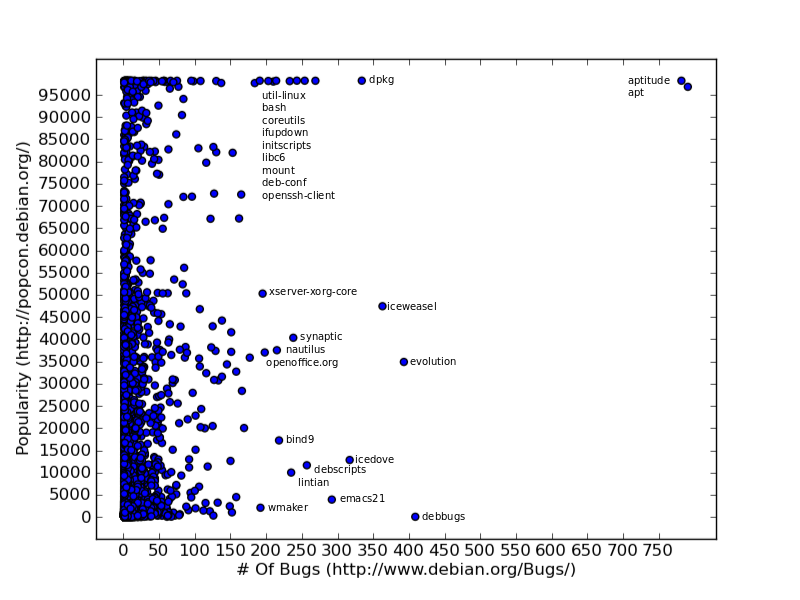
\includegraphics[width=\textwidth]{simulationpics/bugsvspopularity}
  \caption[Bugs v.s. Popularity]{A plot of the bugs a package has compared to its popularity, with notable outliers labeled}
  \label{bugsvspop}
\end{center}
\end{figure}

The first thing to note is that there seems to be very little relationship between the two variables, except the package with the most bug reports is also one of the most used components.
The second thing to note is that the packages with the largest amount of bugs are ``apt'' and ``aptitude'' the two most popular package manages.
This could be because those packages are very buggy, or it could be because problems caused by apt, e.g. trying and failing to install a faulty package, may be reported as a problem with apt. 
The last thing to notice is that there are many less popular components that have many bug reports.
When identifying the purposes of these packages many are used by developers, e.g. emacs21 is a popular text editor to develop in.
The reason for their increased amount of bug reports may be that the users have prior experience and appreciation for the bug reports and the maintenance process, so file more bugs.

Measuring a components likely hood of failure using bug reports is then hypothesised to be not possible,
as a component purpose and a components users may affect the results.
Other methods of finding a components likelihood of failure have not been further explored since this variable was eliminated from the configuration.
Though, we expect this is an intractable problem that is likely impossible to simulate accurately.

\subsection{Further Validation}
The assignment of the configuration variables is a different stage in the validation of this simulation.
Clearly if you create a configuration that is completely unrealistic, the saying ``garbage in, garbage out'' applies to the results.
However, this is not a concern when validating the conceptual model, or the abstract processes.
Further discussion of the validation of the assignment of the configuration variables is in chapter \ref{ubunutsimulation}.

\section{Summary}
{}This chapter has described the abstract definition of the proposed simulation used to study component system evolution.
{}The methodology from Law \cite{Law2005} was used to guide us to a valid and credible simulation.
{}From this methodology we defined a conceptual model of the user, repository and solver and described the implemented processes used to simulate a systems evolution over a time period.
{}It was validated through regular meetings with the core stakeholders, and a survey conducted on subject matter experts.
{}This simulation can, and will, be used to draw meaningful conclusions on component system evolution, though no
